\section{Die Bogenlänge parametrisierter Kurven}
Die Einführung zu diesem Kapitel wird im Unterricht behandelt\dots


% Durchläuft man eine Kurve, so legt man dabei eine gewisse Distanz zurück. Aber wie berechnet man die Länge des zurückgelegten Weges?

% Rufen wir uns dazu in Erinnerung, dass die Momentangeschwindigkeit $\vec{v}(t)$ der parametrisierten Kurve $\vec{r}(t)$ zum Zeitpunkt $t$ dem Tangentialvektor $\vec{v}(t) = \dot{\vec{r}}(t)$ entspricht. So ist intuitiv klar, dass der zurückgelegte Weg zwischen den Zeitpunkten $a$ und $b$ durch das Integral der Schnelligkeit $|\dot{\vec{r}}(t)|$ über dem Intervall $[a, b]$ gegeben ist.

\begin{definition}
    {Bogenlänge einer Kurve}{Bogenlänge}
    Sei $\vec{r}: \, [a,b] \longrightarrow \mathbb{R}^n$ eine parametrisierte Kurve. Dann heisst
    $$L \; = \; \int\limits_{a}^{b} \, |\dot{\vec{r}}(t)| \, dt $$
    die Bogenlänge von $\vec{r}(t)$.
\end{definition}

\begin{bsp}{Bogenlänge eines Halbkreises}{}
    Der Halbkreis vom Radius $R$ in der oberen Halbebene des $\mathbb{R}^2$ mit Zentrum im Ursprung lässt sich auf ganz unterschiedliche Weisen parametrisieren. Wir betrachten hier die beiden Parametrisierungen
    $$\vec{r}_1:[0,1] \longrightarrow \mathbb{R}^2, \;\;\; \vec{r}_1(t) = \begin{pmatrix}
    R \, \cos (\pi \, t) \\ 
    R \, \sin(\pi \, t)
    \end{pmatrix} $$
    %\hspace{0.3cm} \mbox{sowie} \hspace{0.3cm}
   
    \vspace*{12cm}
    \pagebreak
    $$ \vec{r}_2:[0,\pi \, R] \longrightarrow \mathbb{R}^2, \;\;\; \vec{r}_2(t) = \begin{pmatrix}
    R \, \cos (t/R) \\ 
    R \, \sin(t/R)
    \end{pmatrix}$$

    \vspace*{10cm}
\end{bsp}

\begin{bsp}
    {Bogenlänge einer Schraubenlinie}{}
    Betrachten wir die Raumkurve $\vec{r}:\mathbb{R} \longrightarrow \mathbb{R}^3$, $\vec{r}(t) = \begin{pmatrix} 3\cos(t) \\ 3\sin(t) \\ 4t \end{pmatrix}$.
    \begin{center}
        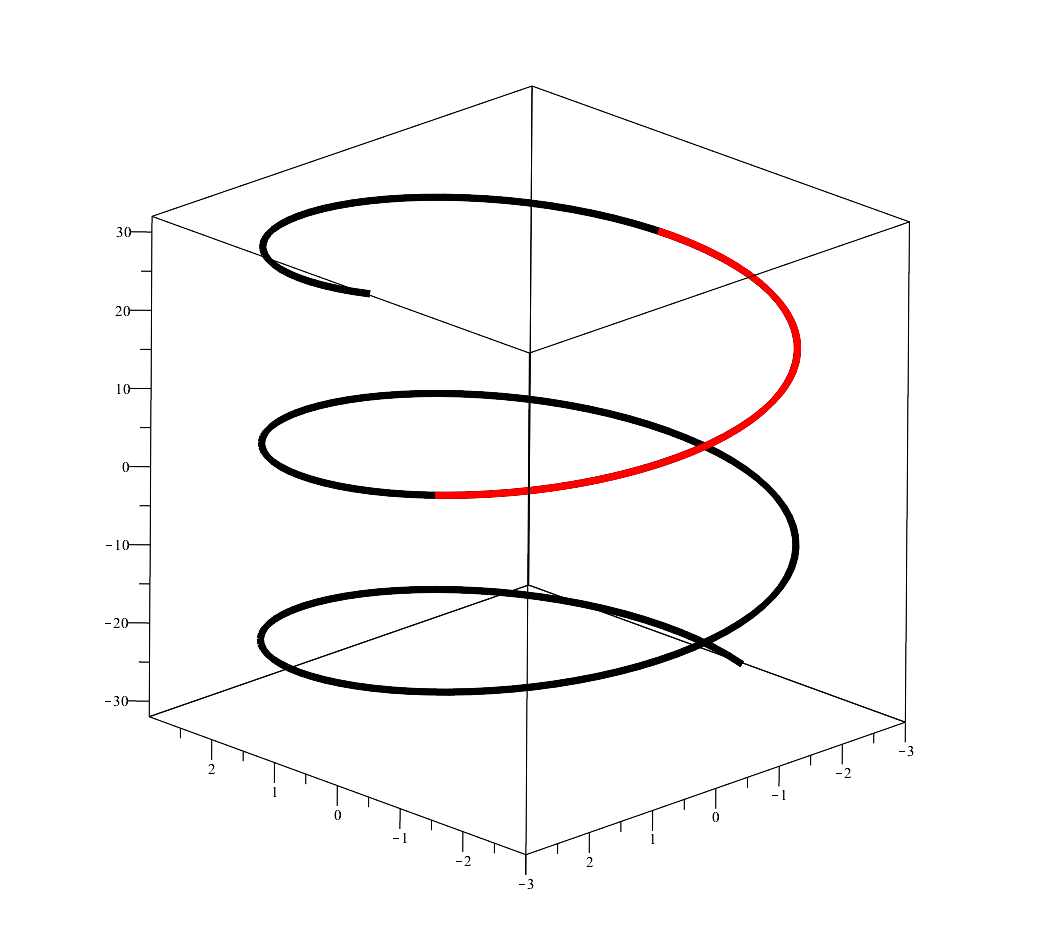
\includegraphics[width=0.5\textwidth]{spiral.png} 
    \end{center}
    Ihre Spur ist eine unendliche Schraubenlinie um die $z$-Achse. Im folgenden soll die Bogenlänge des rot markierten Kurvenstücks berechnet werden. Dieses entspricht dem Teil der Bahn, der zwischen den Zeitpunkten $t_1=0$ und $t_2=2$ durchlaufen wird.
    
\vspace*{10cm}
% Ihre Spur ist eine unendliche Schraubenlinie um die $z$-Achse. Die Momentangeschwindigkeit $\vec{v}(t)$ zum Zeitpunkt $t$
% ist durch $\vec{v}(t) = \dot{\vec{r}}(t) = \begin{pmatrix} -3\sin(t) \\ 3\cos(t) \\ 4 \end{pmatrix}$ gegeben. Ihr Betrag berechnet sich vermöge der trigonometrischen Identität 
% $$\sin^2(t) + \cos^2(t) = 1$$ 
% zu $|\dot{\vec{r}}(t)| = 5$. Daraus folgt, dass die Kurve über dem Parameterintervall $[t_0, t_1] = [0, 2]$ eine Länge von
% $$ L[\, \vec{r} \, _{[0,2]}] = \int\limits_{0}^{2} |\dot{\vec{r}}(t)| \, dt
% = \int\limits_{0}^{2} 5 \, dt
% = \Big[ 5t \Big]_{0}^{2} = 10$$
% besitzt.



\end{bsp}
\pagebreak
\begin{ueb}
{}{}
\begin{enumerate}
    \item Skizzieren Sie die Spuren der folgenden Kurven (Geogebra) und berechnen Sie ihre Bogenlängen:

    \begin{enumerate}
    \item $\vec{r}: [0,\pi] \rightarrow \mathbb{R}^2$, \quad $\vec{r}(t) = \begin{pmatrix} 3 \cdot \cos(t) \\ 3 \cdot \sin(t) \end{pmatrix}$
    \item $\vec{r}: [-1,1] \rightarrow \mathbb{R}^2$, \quad $\vec{r}(t) = \begin{pmatrix} t \\ t^2 \end{pmatrix}$ (Integral numerisch mit dem Taschenrechner berechnen)
    \item $\vec{r}: \left[-\frac{1}{2}, \frac{1}{2}\right] \rightarrow \mathbb{R}^2$, \quad $\vec{r}(t) = \begin{pmatrix} 2t \\ 4t^2 \end{pmatrix}$ (Integral numerisch mit dem Taschenrechner berechnen)
    \item $\vec{r}: [0, 2\pi] \rightarrow \mathbb{R}^2$, \quad $\vec{r}(t) = \begin{pmatrix} \cos(t) \\ \sin(t) \\ t \end{pmatrix}$
    \item $\vec{r}: [0, 2\pi] \rightarrow \mathbb{R}^2$, \quad $\vec{r}(t) = \begin{pmatrix} t- \sin(t) \\ 1-\cos(t) \end{pmatrix}$ (Integral numerisch mit dem Taschenrechner berechnen)
    \end{enumerate}

    \item Ein Ball wird auf einer Abwurfhöhe von \SI{1.60}{\meter} mit einer Anfangsgeschwindigkeit von \SI{12}{\meter\per\second} unter einem Winkel von \SI{30}{\degree} zur Horizontalen abgeworfen. Seine Flugbahn hat dann die Parametergleichung
    \[
        \vec{r}(t) = \begin{pmatrix}
        6\sqrt{3}t \\
        6t - \frac{1}{2} g t^2 + 1.6
        \end{pmatrix}.
    \]
    
    \begin{enumerate}
        \item Berechnen Sie den Geschwindigkeitsvektor zur Zeit $t=0$ und den Beschleunigungsvektor und überprüfen Sie, ob diese zu den Angaben im Text passen.
        \item Berechnen Sie, wie lange es dauert, bis der Ball wieder auf den Boden prallt, und die (Bogen)-Länge der Flugbahn. (Integral numerisch mit dem Taschenrechner berechnen)
    \end{enumerate}


    \item Das Integral, mit dem man die Bogenlänge berechnet, ist ein Spezialfall der skalaren Kurvenintegrale (oder Kurvenintegrale 1. Art). Schauen Sie sich die beiden Videos dazu an, die im Moodle-Kurs verlinkt sind, und berechnen Sie das folgende Integral
    $$ \oint_K f\, ds$$
    wobei $K$ der Einheitskreis und $f$ die Funktion $f(x,y)=5x^2+5y^2$ ist. 

    \item Die Masse \( m \) eines Drahtes soll in Abhängigkeit eines Parameters \( \lambda \) berechnet werden. Dabei ist die ortsabhängige Dichte \( \rho \) durch die Funktion 
    \[ \rho(x,y,z) = \lambda(x + z) \] 
    gegeben.
    
    Der Draht folgt dabei der Kurve \( \mathcal{C} \) mit:
    \[
    \mathcal{C} : \, \vec{r}(t) = \begin{pmatrix} 
        \frac{2}{3}t^3\\
        t^2 \\
        t+1
    \end{pmatrix}, \quad 0 \leq t \leq 1
    \]
    
\end{enumerate}

\end{ueb}
\clearpage
\emph{Lösungen:}
\begin{enumerate}
    \item Bogenlängen berechnen
    \begin{enumerate}
        \item Halbkreis mit Radius 3: Bogenlänge $L=3\pi$.
        \item Normalparabel. Bogenlänge $L\approx 2.958$ (Das bestimmen der Stammfunktion ist in diesem Fall nicht einfach...)
        \item Es ist die gleiche Kurve wie bei (b) bloss anders parametrisiert: Bogenlänge $L\approx 2.958$ (Das bestimmen der Stammfunktion ist in diesem Fall nicht einfach...)
        \item Schraubenlinie. $L=2\sqrt{2}\pi$
        \item Zykloide. $L=8$
    \end{enumerate}
    \item Ball
    \begin{enumerate}
        \item es ist: 
        \[
            {\vec{v}(t)} = \begin{pmatrix}
            6\sqrt{3} \\
            6 - gt
            \end{pmatrix}
            \Rightarrow
            \vec{v}(0) = \begin{pmatrix}
                6\sqrt{3} \\
                6 
                \end{pmatrix}
            =
            12\begin{pmatrix}
                \frac{\sqrt{3}}{2} \\
                \frac{1}{2}
                \end{pmatrix}
            =
            12\begin{pmatrix}
                \cos(\SI{30}{\degree}) \\
                \sin(\SI{30}{\degree})
                \end{pmatrix}
        \]
        Das passt!

        Und für die Beschleunigung:
        \[
            {\vec{a}(t)} = \begin{pmatrix}
            0 \\
            - g
            \end{pmatrix}
        \]
        Das passt auch!
        \item Aufprallzeitpunkt: $y=0 \Rightarrow t \approx 1.45$ (negative Lösung ergibt im Kontext keinen Sinn)
        
        Länge der Flugbahn: $L\approx 16.23$
        
    \end{enumerate}
    \item Kurvenintegral erster Art:  $$ \oint_K f\, ds = 10\pi $$
    \item Integriere die Dichtefunktion entlang der Kurve:
    $$m = \int_C \rho \, ds = \int_0^1 \rho(r(t)) \cdot  |\dot{\vec{r}}(t)| \, dt = \frac{55}{18}\lambda$$
\end{enumerate}